\documentclass{standalone}
\usepackage{pgfplots,pgfplotstable}
\begin{document}
\begin{tikzpicture}

\definecolor{darkgreen}{RGB}{31,182,83}

\begin{axis}[
    view={50}{40},
    samples=3,
    %domain=-4:4,
    %samples y=0, ytick={1,...,4},
    %zmin=0,
    %y dir=reverse,
    %yticklabels={,,},
    %zticklabels={,,},
    %ytick style={draw=none},
    %ztick style={draw=none},
    %xtick style={draw=none},
    %z axis line style={draw opacity=0},
    %x axis line style={draw opacity=0},
    %axis y line = middle,
    area plot/.style={
        fill opacity=0.75,
        %draw=orange!80!black,thick,
        %fill=orange,
        draw=darkgreen!80!black,thick,
        fill=darkgreen,
        mark=none,
    }
]
%\addplot3 [area plot] graphics {
\addplot3 [area plot] graphics[xmin=0,ymin=0,xmax=0,ymax=96,zmin=0,zmax=96] {
placeholder2.png
};
%\addplot3 [area plot] coordinates {
%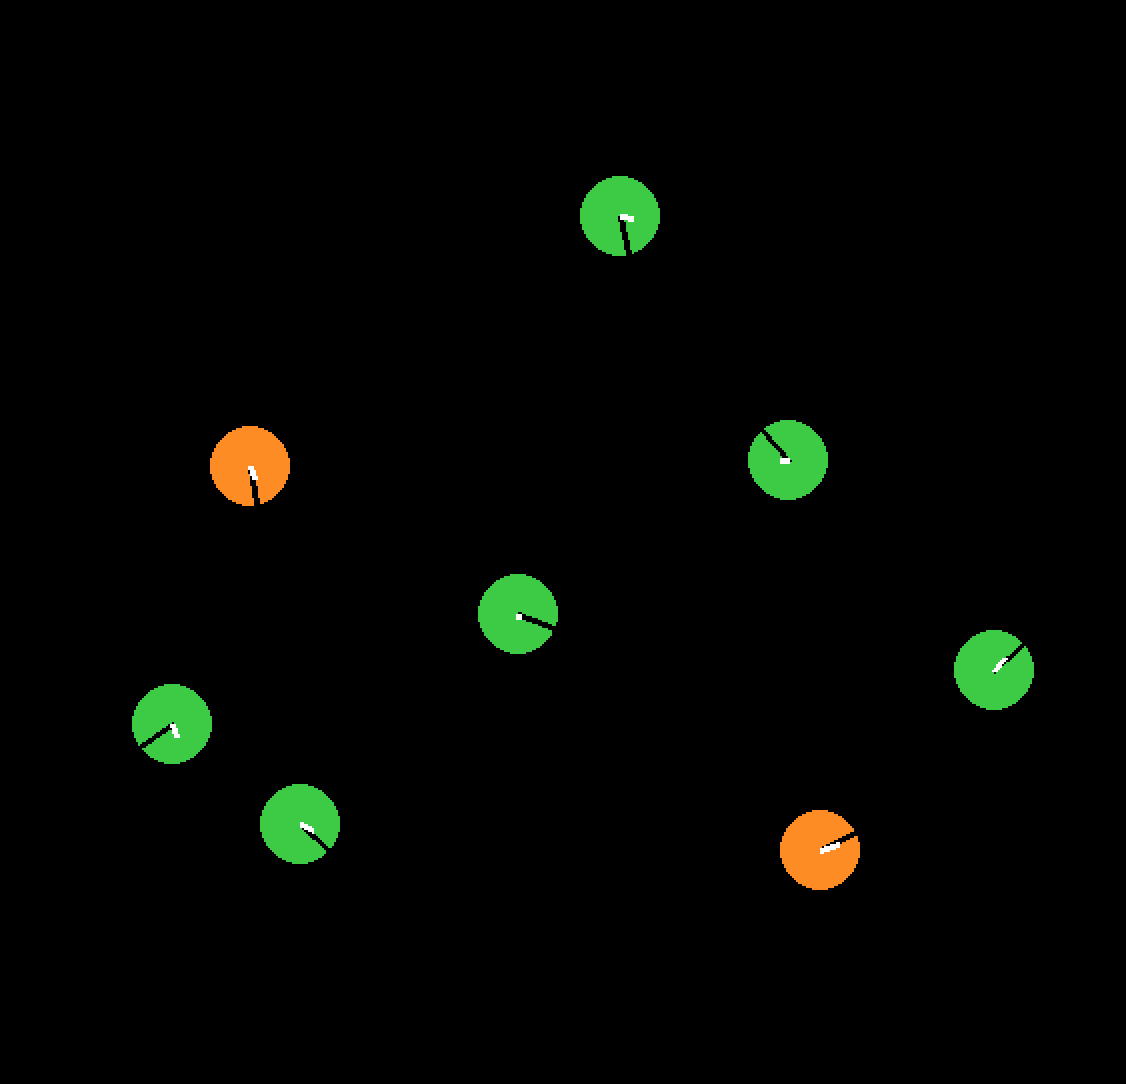
\includegraphics[width=3cm]{placeholder}
%};


%\pgfplotsinvokeforeach{4,3,...,1}{
%    %\addplot3 [area plot] table [x expr=\coordindex, y expr=#1, z=plot#1] {\dummydata};
%    \addplot3 [area plot] table [x expr=\coordindex, y expr=#1, z=plot#1] {\dummydata};
%}
\end{axis}
\end{tikzpicture}

\end{document}
